\chapter{Introduction}

\section{Context}

Machine learning (\acrshort{ml}), the sub-field of \acrfirstit{ai} which is concerned with how to make a computer learn from data, has been through quite a journey since its inception in the 1940s and 1950s. From a small research domain, it has grown into a massive rapidly-developing field of research and applications with ramifications in many branches of science and technology. This growth is not surprising in a world where computers become more and more powerful and data, the bread-and-butter of \acrlong{ml}, is becoming increasingly collectable, structured, available and queryable. Applications of \acrlong{ml} are as varied as they are numerous: spam filtering, fraud detection, face recognition, self-driving cars, robotics and automation, medical data analysis and diagnosis, simulation in particle physics... to name only a few. While it has already revolutionized many domains, \acrlong{ml} research has still a bright future ahead. In the last decade only, several new family of techniques have been (re-)discovered and have enabled unexpectedly-fast progress (\eg \acrlong{dl}, \acrlong{cnn}, \acrlong{gan}, transformers). One can only expect that the next ground-breaking \acrshort{ml} method is on the brink of being discovered in a research lab somewhere around the world. Aside from that, research is still ongoing of many fronts such as understanding, applying or improving existing methods.

Medicine is among the numerous fields where \acrlong{ml} is showing great promises. Although often misrepresented in the mainstream media as a tool that will eventually replace practitioners, the real potential of \acrlong{ml} in medicine actually lies in its capacity to become a strong, resilient and consistent assistant to the physicians \parencite{rajkomar2019machine}, assisting them for tasks ranging from diagnosis and analysis to paperwork. Rather than replacing physicians, an \acrshort{ai}-based diagnosis system would be able to complement their opinion and advise them based on experiences of millions of other patients and colleagues. Moreover, such a system would be able to produce these advice based on a very large number of parameters and sources of data that a human could not realistically consider (imaging, written reports, laboratory values, vital signs). However, the road to an \acrshort{ai}-assistant is still long and many questions and challenges have yet to be addressed. From a scientific standpoint, current research mostly focuses on improving solutions for tasks of significantly smaller scale and scope (\eg outlining organs in x-rays, detecting disease in \acrshort{ct}-scans, classifying skin cancer as malignant or benign). Many recent contributions, some of which the generalization can be questioned \parencite{nagendran2020artificial}, have claimed to have matched or surpassed human experts accuracies by applying \acrlong{ml} methods on different medical tasks. Whereas progress is certain, many challenges have yet to be solved. 

One of these major challenges is \textit{data scarcity}. Not that data itself is lacking as \cite{pramanik2019healthcare} reported that the amount of health data stored worldwide could reach 2,258 exabytes in 2020. What is scarce is actually data that is at least partially annotated and of good-enough quality to be used to train \acrlong{ml} models. Data scarcity has many causes: privacy concerns prevent sharing patient data, the annotation process is time-consuming and expensive, \etc. This is aggravated by the fact that recent \acrlong{ml} methods (\ie \acrlong{dl}) require a significant amount of data to perform optimally.

In this thesis, we are interested in one specific field of medicine: \acrfirstit{dp}. Microscope have been used in medicine to analyze samples (\eg cells, tissue or blood) since the 17th century \parencite{hajdu2002first} but recent technological progress has enabled the digitization of microscope glass slides into images called \acrlong{wsi}s (\acrshort{wsi}). Digital pathology concerns all the aspects of acquiring, managing, sharing and interpreting these \acrshort{wsi}s \parencite{doolan2019whatisdp}. With the help of image management systems, modern visualization tools like Cytomine \parencite{maree2016collaborative} and image analysis algorithms, \acrshort{wsi}s have the potential to revolutionize the daily work of pathologists and biologists but the transition process is complex and expensive. Therefore, only a few hospitals and facilities took the leap towards a full digital environment (\eg \cite{stathonikos2013going, eloy2021digital, temprana2022digipatics}). Among the greatest promises of \acrlong{dp} is the possibility to automate diagnosis tasks with computer vision techniques including \acrlong{ml} \parencite{ciompi2021editorial}. Such automation would not only accelerate the diagnosis process but could also improve its accuracy by delegating time-consuming and tedious but simple tasks to algorithms (\eg counting cells, measuring area of tumor) therefore allowing practitionners to focus on the challenging aspects of their work and ultimately improving patient care and treatments. The use of such techniques would also contribute to accelerating drug and pathology research relying on \acrlong{wsi} analysis. 

\begin{figure}
  \centering
  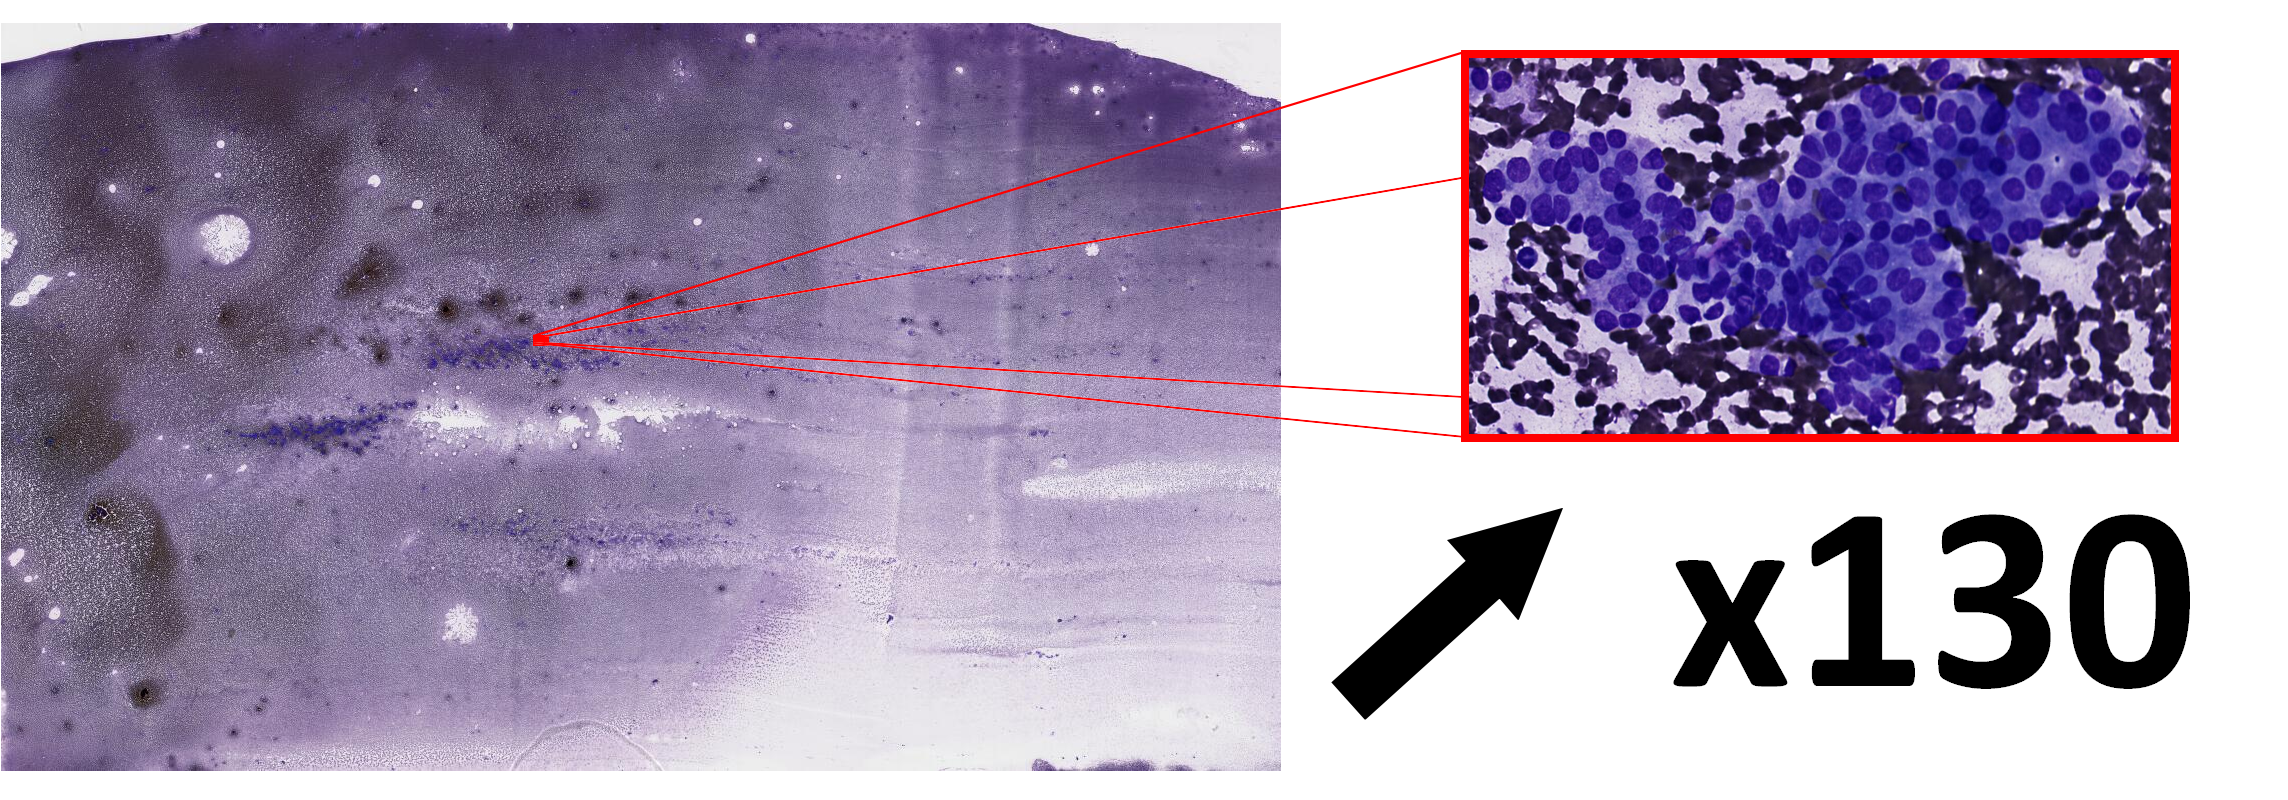
\includegraphics[scale=0.25]{intro/whole-slide-dim.png}
  \caption{A typical \acrlong{wsi} of size 163840 $\times$ 95744 pixels and file size of 2.3 gigabytes. To the left is the original slide and to the right is a structure of interest at zoom level $\times130$ (size in pixels: 1354 $\times$ 736)}.
  \label{fig:intro:wsi}
\end{figure}

The subfield of \acrlong{dp} focusing on automating the analysis of pathology data is called \acrfirstit{cpath} and faces many interesting challenges. A \acrshort{wsi} is typically a very large image that can reach few billion pixels at maximum zoom level (see Figure \ref{fig:intro:wsi}, a single file can weight several gigabytes) therefore making classical computer vision methods inapplicable without adaptation. The image content is usually complex which excludes the use of naive computer vision methods. This explains why \acrlong{ml} is currently so popular among \acrlong{cpath} researchers because of its ability to cope with the complexity by automatically learning from data. However, efficient use of \acrlong{ml} is hampered by data scarcity of which the field is not spared since billion-pixels images are as tedious to analyze as to annotate exhaustively, even for trained pathologists. The data scarcity problem is made worse by the variability introduced by the transformation process of a biological sample into a slide and then into a \acrlong{wsi}.

\section{Contributions and outline}

In this thesis, we explore different ways of tackling data scarcity in \acrlong{dp} using \acrlong{dl}, a sub-field of \acrlong{ml} which focuses on deep neural networks. Our contributions leverage \acrfirst{tl}, \acrfirst{mtl} and self-training which we apply to the tasks of image classification and segmentation. Our contributions are as follows. The manuscript is structured in three parts which are preceeded by this introduction.

Part \ref{part:background} introduces \acrlong{ml} and \acrlong{dp}. Chapter \ref{chap:backml} focuses on \acrlong{ml} and presents the different concepts and techniques used throughout this thesis. It is not intended to explain the matter in depth but rather to give sufficient background for a reader with a basic knowledge of \acrlong{ml} to understand the contributions. This chapter also presents works related to ours. More precisely, we discuss how similar techniques are used for general purpose problems (\ie not specific to medical imaging). Chapter \ref{chap:backdp} focuses on \acrlong{dp} and presents the field from the perspective of a computer scientist. It presents how a biological sample is transformed and ultimately becomes a \acrlong{wsi} in order to explain how this crucial preparation step can impact the image analysis down the line. We also present three example diagnosis tasks that would greatly benefit from automation with computer vision techniques. We also introduce the challenge that is data scarcity more in depth and present works related to ours. Unlike in Chapter \ref{chap:backml}, the related works are focused on medical and pathology application of methods similar to ours.

Part \ref{part:transfer} presents our first and second contributions which are both related to \acrlong{tl}. In Chapter \ref{chap:comp}, we first review, compare and study different deep \acrlong{tl} techniques using 8 classification datasets in order to evaluate the viability and best practices of \acrlong{tl} in \acrlong{dp}. We show that using neural networks pre-trained on a dataset unrelated to digital pathology (\ie ImageNet \parencite{deng2009imagenet}) is indeed interesting compared to training a network from scratch. We also draw guidelines from our experiments on how the transfer should be performed. In Chapter \ref{chap:mtask}, we then propose a \acrlong{mtl} architecture and training scheme for pre-training a network based on an ensemble of potentially-small datasets rather than a single large dataset. We use these in order to pre-train a neural network on 22 classification \acrlong{dp} datasets and show that our resulting models yield competitive results compared to networks pre-trained on ImageNet. 

Part \ref{part:segmentation} presents our third contribution on self-training in an imperfect dataset setting. We study how sparse annotations can be exploited to improve a segmentation model by using a technique called self-training where a \acrlong{ml} model is both trained and used to predict missing annotations in the dataset. We show that our approach is indeed able to make efficient use of sparse annotations and that it is not always necessary to exhaustively annotate a dataset to obtain competitive segmentation performance. 

The manuscript ends with Chapter \ref{chap:conclusions} which presents our conclusions and discussion of future works.
% Part \ref{part:software} presents our software contributions including Biaflows and SLDC.

\section{Publications and code}

This thesis is based on the following publications:
\begin{itemize}
  \item \fullcite{mormont2018comparison}
  \item \fullcite{mormont2020multi}
  \item \TODO{publication selftraining}
\end{itemize}

During the course of the PhD, I have contributed to the development of Biaflows, a platform designed for standardized benchmarking of bioimage analysis workflows. This work is not presented in the thesis but resulted in the following publication and open-source project: 
\begin{itemize}
  \item \AtNextCite{\defcounter{minnames}{2}}\fullcite{rubens2020biaflows}
\end{itemize}

I have frequently used and updated the SLDC framework created from my master thesis throught the years to support my implementations:
\begin{itemize}
  \item \fullcite{mormont2016sldc}
\end{itemize}

The code and models for our publications are also publicly available online with permissive licenses:
\begin{itemize}
  \item Chapter \ref{chap:mtask}: \url{https://github.com/waliens/multitask-dipath}
  \item Chapter \ref{chap:strain}: \TODO{self-training repo}
\end{itemize}

